\documentclass[aspectratio=169,usenames,dvipsnames]{beamer}
\usepackage{preamble}
\title{Coding for Humanities, week 3}

\begin{document}

\begin{frame}
 \titlepage
\end{frame}

\begin{frame}{Last week}
    Lists

    Conditions

    Loops
\end{frame}

\begin{frame}{Plan for today}
 \tableofcontents
\end{frame}


\section{Dictionaries}
\frame{\tableofcontents[currentsection]}

\begin{frame}
    \begin{itemize}
        \item Lists are useful when data has a natural order: \\
            items are referred by their position
        \pause
        \item What if we have lots of data,
            but we need to find it some other way?
    \end{itemize}

    \begin{block}{Example}
    Finding words in a dictionary

    Too many words to consider one-by-one

    However, due to organization (sorted), can find words quickly
    \end{block}
\end{frame}


\begin{frame}[fragile]{dictionaries}
    \begin{definition}
        A dictionary stores pairs of values (key, value),
        such that we can quickly find a value given a key.
    \end{definition}
Example, a phone book:
\begin{lstlisting}
>>> coworkers = {'John': 123, 'Mary': 456, 'Alice': 789}
>>> coworkers['Mary']
456
>>> coworkers['Bob'] = 124
\end{lstlisting}

% Explanation of hash tables:
% https://dev.to/a_sandrina_p/learning-hash-tables-with-drawings-99o
\end{frame}

\begin{frame}{Properties of dictionaries}
A dictionary is a mapping of keys to values.

    \begin{itemize}
        \item Looking up a key is fast
        \item Keys must be immutable (e.g., numbers or strings).
        \item Values can be anything.
        \item Keys are always unique;
            re-using a key will overwrite the previous value.
    \end{itemize}
\end{frame}

\begin{frame}[fragile]{Looping over dictionaries}
Looping over a dictionary returns only the keys:
\begin{lstlisting}
data = {'a': 0, 'b': 1}
for key in data:
    print(key)
    print(data[key])
\end{lstlisting}

\pause
Often want both the key and the value:
\begin{lstlisting}
for key, value in data.items():
    print(key)
    print(value)
\end{lstlisting}
\end{frame}


\section{Data organization}
\frame{\tableofcontents[currentsection]}

\begin{frame}[fragile]{Combining lists and dictionaries}
Lists and dictionaries can contain any kind of value

Even other lists and dictionaries!

\begin{lstlisting}
>>> x = [[0, 1], [2, 3]]
>>> x[0]
[0, 1]
>>> x[0][0]
[0]
\end{lstlisting}
\end{frame}

\begin{frame}[fragile]{Practical example}
Two ways of organizing a collection of books:
\begin{lstlisting}
>>> books = ['Tolstoy - War and Peace', 'Tolstoy - Anna Karenina',
...     'Dostoevsky - Crime and Punishment',
...     'Dostoevsky - Brothers Karamazov']
\end{lstlisting}

\pause
\begin{lstlisting}
>>> books = {'Tolstoy': ['War and Peace', 'Anna Karenina'],
...     'Dostoevsky': ['Crime and Punishment',
...         'Brothers Karamazov']}
>>> books['Tolstoy']
...
\end{lstlisting}
The latter has the advantage of easily being able to
select the works by a particular author.
\end{frame}

\begin{frame}{Algorithms + Data structures = Programs}
    \begin{columns}
        \column{0.5\linewidth}
            \begin{itemize}
                \item Thinking of how to organize your data is an important
                    first step in designing a program
                \item The right organization may make the rest of the design
                    obvious
                \item Often a trade-off: particular choices may make one thing
                    easy and another hard
            \end{itemize}
        \column{0.5\linewidth}
            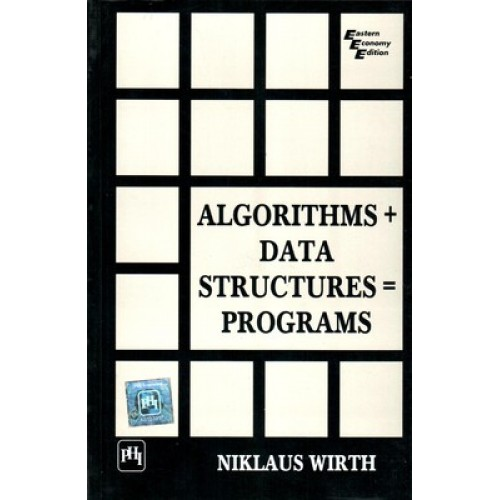
\includegraphics[height=0.8\textheight]{fig/wirth}
    \end{columns}
\end{frame}




\section{Defining functions}
\frame{\tableofcontents[currentsection]}

\begin{frame}{Motivation}
    \begin{itemize}
        \item We've used builtin functions (print, len, sorted);\\
            now we'll see how to make our own functions
        \item Why? Modularity; i.e., break down programs into smaller components
            \begin{itemize}
                \item Can create larger, more complex programs
                    from readily understandable building blocks
                \item Functions encapsulate complexity;
                    don't need to understand how a function works to use it
                \item Components are re-usable;
                    write once, use many times
            \end{itemize}
    \end{itemize}
\end{frame}

\begin{frame}[fragile]{Defining functions}
    Basic syntax:
\begin{lstlisting}
def function(param1, param2, ...):
    # do something with parameters
\end{lstlisting}

    A function definition has\dots
    \begin{itemize}
        \item A name
        \item A fixed number of parameters (may be zero)
        \item An indented block of code
    \end{itemize}
\end{frame}

\begin{frame}[fragile]{Defining a function does not run it}
    \begin{itemize}
        \item Executing a \texttt{def} statement does not run the code!
        \item The function is stored along with its name
        \item Function must be called to run it
    \end{itemize}
    Example:
\begin{lstlisting}
def greeting():
    print('Hello!')

greeting()
\end{lstlisting}
\end{frame}

\begin{frame}[fragile]{Function arguments}
    \begin{definition}
        A \structure{parameter} is a value expected by a function

        An \structure{argument} is a particular value for a parameter
            when calling a function
    \end{definition}

    \begin{itemize}
        \item Can pass data to functions using arguments
        \item Below, the argument \texttt{'John'} is assigned
            to the parameter \texttt{name} when the function is called
        \item Arguments have a specific order
        \item When calling a function, must use correct number of arguments
    \end{itemize}
Example:
\begin{lstlisting}
def greeting(name):
    print('Hello', name)

greeting('John')
\end{lstlisting}
\end{frame}

\begin{frame}[fragile]{Returning results}
    \begin{itemize}
        \item A function does not need to return a result \\
            In this case, 
            \begin{itemize}
                \item the function is used for its \emph{effect};\\
                    it does something (e.g., print text on screen)
                \item The value \texttt{None} is implicitly returned
            \end{itemize}
        \item Use \texttt{return ...} to give a result back to the caller
        \item May occur anywhere in the function
    \end{itemize}

Example:
\begin{lstlisting}
def average(values):
    if len(values) == 0:
        return None
    return sum(values) / len(values)
\end{lstlisting}
\end{frame}

\begin{frame}{Summary}
    \begin{itemize}
        \item Break programs down into functions to make them easier
            to understand.
        \item Define a function using \texttt{def} with a name, parameters,
            and a block of code.
        \item Defining a function does not run it.
        \item Arguments in call are matched to parameters in definition.
        \item Functions may return a result to their caller using return.
    \end{itemize}
\end{frame}




\section{Cleaning text}
\frame{\tableofcontents[currentsection]}
\begin{frame}{Goal: text $\rightarrow$ words}
    For basic text analysis,

    want to consider only word frequencies of a text

    \pause
    Therefore:
    \begin{enumerate}
        \item Identify words
        \item Simplify text, remove non-words
        \item Count words to get frequencies
    \end{enumerate}
\end{frame}

\begin{frame}[fragile]{Upper and lower case}
    \begin{itemize}
        \item To the computer, these
            are three completely different words!

            \texttt{'John', 'john', 'JOHN'}
        \item Often, we don't want to make this distinction when counting
        \item One solution: case folding
    \end{itemize}
    \pause
\begin{lstlisting}
text = 'HeLlO WoRlD'
cleaned = text.lower()
\end{lstlisting}
\end{frame}

\begin{frame}[fragile]{Punctuation}
    \begin{itemize}
        \item Similarly, punctuation should be separated from words
        \item Or should be eliminated completely
        \item Can use functionality similar to "find \& replace" for this
    \end{itemize}
    \pause
\begin{lstlisting}
text = "Forsooth, 'tis true!"
text = text.replace('!', '')
text = text.replace(',', '')
\end{lstlisting}
\end{frame}

% mention regular expressions

\begin{frame}{Summary}
\end{frame}

% parsing a simple text file line-by-line, e.g. subtitles?

% explain complexity



\begin{frame}{Intermezzo: How to solve problems}
	\begin{columns}
		\column{0.5\linewidth}
			The Feynman algorithm:
			\begin{enumerate}
				\item Write down the problem.
				\item Think real hard.
				\item Write down the solution.
			\end{enumerate}

			\vspace{1em}
			due to Richard Feynman, Nobel-prize winning physicist \dots
		\pause
		\column{0.5\linewidth}
			Pólya (1945), How to solve it:

			\begin{enumerate}
				\item First, you have to understand the problem.
				\item After understanding, make a plan.
				\item Carry out the plan.
				\item Look back on your work. How could it be better?
			\end{enumerate}

			\begin{block}{Stuck?}
			If you can't solve a problem,
			then there is an easier problem you can solve:
			find it.
			\end{block}
	\end{columns}
\end{frame}


\begin{frame}{Background reading}
    \begin{itemize}
        \item Downey ch.\ 3, 6, 11, 14
        \item and/or Zelle sec.\ 5.9, ch.\ 6
        \item Watch youtube tutorials of "Hacking the Humanities" episode 10--12:
            \url{https://www.youtube.com/playlist?list=PL6kqrM2i6BPIpEF5yHPNkYhjHm-FYWh17}
    \end{itemize}
\end{frame}
\end{document}
